\documentclass[main.tex]{subfiles}

\begin{document}
\sloppy


\vspace{1.0cm}

\chapter{Simulatore di parcheggio}\label{sec:Simulazione}

Prima del mio arrivo nel Gamification Lab, il mio collega Marco Wang per la sua tesi triennale \cite{TesiMW}, aveva creato una prima versione di un bot che simulava il comportamento di un taker, con l'obbiettivo di verificare l’efficacia e la validità del sistema di match. \newline
Questa prima versione di simulazione era però migliorabile aggiungendo un secondo tipo di bot per simulare il comportamento di un giver ed una interfaccia per mostrare il match in tempo reale. \newline
In questo capitolo, si espone la nuova versione del simulatore di parcheggio tra bot con tutte le aggiunte esposte sopra, nonché il tema principale del mio tirocinio.  


\section{Funzionamento}
Come spiegato nella sezione \ref{Funzionamento}, la simulazione sfrutta il meccanismo di match, il quale prevede due ruoli:
\begin{itemize}
    \item \textbf{Taker}: l'utente che vuole occupare un parcheggio;
    \item \textbf{Giver}: l'utente che sta lasciando un parcheggio.
\end{itemize}
Vogliamo quindi realizzare una simulazione dove i bot che simulano il comportamento di un giver aspettano parcheggiati che avvenga un match con un bot che simula il comportamento di un taker.\newline
Per fare in modo che tra due bot inizi un match, un bot parcheggiato dovrà inviare al server una richiesta contenente la sua posizione e l'orario di partenza, diventando così un giver, mentre un secondo bot che ha il compito di parcheggiare invia al server una richiesta con la sua posizione, il raggio di ricerca e l'orario desiderato per parcheggiare, diventando così un taker.\newline
Il server è continuamente alla ricerca di possibili match, cercando di abbinare ogni taker con un giver. Per abbinare due bot ed iniziare così un match, il server controlla se la posizione di un giver rientra nell'area di ricerca di un taker e se i loro orari desiderati di \say{sparcheggio} e parcheggio coincidano. Se le due condizioni precedenti sono soddisfatte, viene inizializzato un match tra i due bot. \newline
Per avere il maggior numero di match possibili, il server divide le richieste in slot temporali da 15 minuti. Quindi, quando un taker o un giver invia il suo orario desiderato, esso verrà inserito nello slot di 15 minuti corretto. Ad esempio, se un giver inviasse come orario di partenza 11:43, il server lo inserirà nello slot temporale delle 11:45 mentre uno che imposta come orario di partenza 11:48, verrebbe inserito nello slot delle 12:00.


\section{I Bot}
Abbiamo quindi bisogno di due tipi di bot che simuleranno il comportamento dei due tipi di utenti, inviando richieste al server per iniziare e completare un match.\newline
Il funzionamento di un bot è diviso in due parti :
\begin{itemize}
    \item {Configurazione}
    \item {Simulazione}
\end{itemize}
Mentre la prima fase di configurazione avviene in maniera iterativa per tutti i bot necessari, la seconda fase di simulazione avviene in modo asincrono. Questo significa che tutti i bot eseguono la simulazione in parallelo sfruttando le \textbf{goroutine} \cite{Goroutine}, le quali rappresentano i thread in Go.

\subsection{Configurazione}
Per far partire il programma dei taker bot bisogna usare il seguente comando: 
\begin{lstlisting}[language=python]
go run ./cmd/taker-bot --config-path ./demo/takerbot.yml
\end{lstlisting}
Similmente, per far partire i giver bot, si utilizza quest'altro comando:
\begin{lstlisting}[language=python]
go run ./cmd/giver-bot --config-path ./demo/giverbot.yml
\end{lstlisting}
Una volta in esecuzione inizia per entrambi la fase di inizializzazione, nella quale viene caricato il file di configurazione passato nei parametri dei comandi sopracitati. Questi file contengono tutte le informazioni necessarie riguardo la creazione dei bot e per assicurare la corretta esecuzione del programma. Queste informazioni sono divise in 6 categorie:

\begin{itemize}
    \item \textbf{Bot}: contiene il numero di bot ed il nome che avranno;
    \item \textbf{Car}: contiene tutte le informazioni necessarie alla creazione e personalizzazione delle macchine che i bot useranno;
    \item \textbf{Header}: contiene gli header delle richieste HTTP che verranno utilizzate; 
    \item \textbf{Location}: contiene le coordinate da cui un nuovo bot inizia ad operare ed il loro raggio d'azione;
    \item \textbf{Time}: contiene informazioni temporali come l'intervallo di tempo con cui opera il server e, solo per il taker, il tempo massimo e minimo che dovrà attendere un bot per percorrere un tratto di strada (vedi \ref{follow-path});
    \item \textbf{Host}: contiene l'url al quale fare le richieste e i file in cui salvare i bot creati.
\end{itemize}

\lstinputlisting[language=Python]{Code/Simulazione/config-file.yml}

\subsection{Il file CSV}
Per non dover creare nuovi bot ad ogni simulazione, quelli creati in una simulazione verranno riciclati per svolgere anche le successive. Per fare ciò, sfrutteremo due file CSV, uno per ogni tipo di bot, all'interno dei quali salveremo ogni bot creato.\newline
Nel file CSV dei giver bot, verranno memorizzati l'id del bot e quello della sua macchina mentre per i taker bot, oltre ai due id precedenti, anche la latitudine e la longitudine di partenza. \newline
Per dare anche un senso di continuità e realismo alle simulazioni, i bot delle due categorie verranno continuamente scambiati (salvando le loro informazioni nel file dell'altra categoria). Questo significa che, ad esempio, una volta che un giver avrà lasciato il suo parcheggio, le sue informazioni verranno salvate nel file CSV dei taker bot, diventando così un taker che partirà dalle coordinate da cui ha appena \say{sparcheggiato}. Al contempo, una volta che un taker bot avrà occupato il parcheggio lasciato da un giver, salverà le sue informazioni nel file CSV dei giver bot, diventando a sua volta un giver.

\begin{figure}[H]
    \centering
    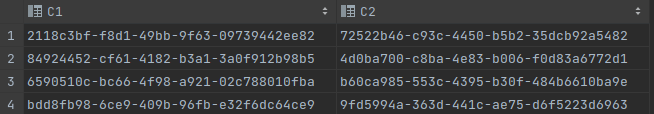
\includegraphics[width=1\linewidth]{img/simulazione/giverbot/giver-CSV.png}
    \caption{File CSV dei giver}
    \label{fig:giverbot csv}
\end{figure}
\begin{figure}[H]
    \centering
    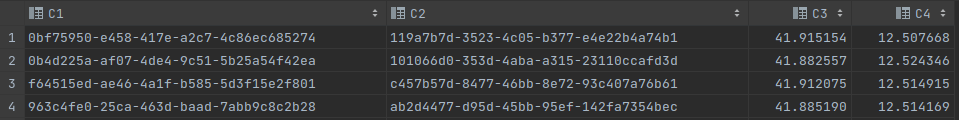
\includegraphics[width=1\linewidth]{img/simulazione/takerbot/taker-CSV.png}
    \caption{File CSV dei taker}
    \label{fig:takerbot csv}
\end{figure}

\subsection{Giver Bot}
Il giver bot è il bot che simula il comportamento di un giver. Questo programma utilizza, per rappresentare un singolo bot, una struttura che raccoglie tutte le informazioni utili per ogni bot. Tra queste informazioni troviamo il suo nome, il suo id, l'id della sua macchina, lo schedule con il quale ha cercato un match, il timeslot in cui ha trovato un match e le coordinate alle quali ha parcheggiato.

\lstinputlisting[language=go]{Code/Simulazione/GiverBot/giver-struct.go}

\subsubsection{Creazione}\label{fig:giver create}
Una volta caricato il file di configurazione viene inizializzato il logger e viene letto il file CSV in cui vengono memorizzati tutti i giver bot creati fin'ora. \newline
Se all'interno del file CSV non dovessero esserci abbastanza bot per raggiungere il numero richiesto nel file di configurazione, vengono creati nuovi bot tramite chiamate API, salvandoli nel file CSV per riutilizzarli in seguito.

\lstinputlisting[language=go]{Code/Simulazione/GiverBot/giver-create.go}
Per permettere un'esecuzione infinita della simulazione, da questo punto in poi tutto il codice sarà in un for infinito, all'interno del quale verranno caricati sempre nuovi bot che svolgeranno indipendentemente la loro simulazione.

\subsubsection{Caricamento} \label{fig:giver load}
Una volta creati i bot mancanti al raggiungimento della quantità richiesta, si passa alla fase di caricamento. In questa fase vengono caricati dal file CSV tutti i bot richiesti, ottenendo le informazioni di ognuno tramite chiamate API. \newline

\lstinputlisting[language=go]{Code/Simulazione/GiverBot/giver-load.go}
Essendo un giver bot, è necessario che il bot sia anche parcheggiato prima di iniziare la simulazione. Per questo motivo vengono generate delle coordinate casuali all'interno dell'area specificata nel file di configurazione. Non vogliamo però che il bot parcheggi in un edificio ma solo in un vero parcheggio ai lati di una strada in cui è possibile parcheggiare.\newline
Per trovare un parcheggio che risponda ai nostri requisiti, vengono eseguite delle richieste API ad OpenStreetMap \cite{OpenStreetMap}, il quale ci restituirà le coordinate di tutte le strade sulle quali è possibile parcheggiare una macchina vicine alle coordinate casuali che abbiamo appena generato. Se OpenStreetMap non dovesse aver trovato nessuna strada valida vicino alle nostre coordinate, vengono generate delle nuove coordinate e fatta una nuova richiesta fino al trovare un parcheggio valido.

\lstinputlisting[language=go]{Code/Simulazione/GiverBot/openStreetMap.go}
Ora che i giver bot sono stati creati e parcheggiati è finalmente possibile iniziare la simulazione nella quale ogni bot agirà indipendentemente dagli altri giver. \newline
In questo punto creiamo anche un canale per catturare i segnali SIGKILL e SIGINTERRUPT così che la simulazione non possa essere interrotta durante la sua esecuzione ma solo una volta che tutti i bot hanno terminato il loro match. \label{fig:giver start}

\lstinputlisting[language=go]{Code/Simulazione/GiverBot/giver-start.go} 


\subsubsection{Simulazione del giver}
\begin{figure}[H]
    \centering
    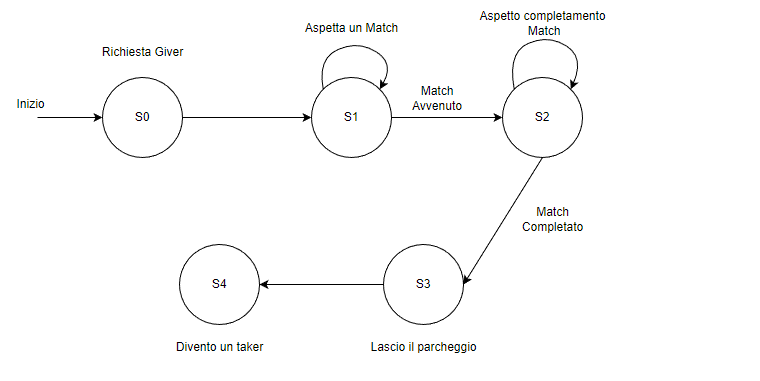
\includegraphics[width=1.2\linewidth]{img/simulazione/giverbot/giverBot-simulazione.png}
    \caption{Automa della simulazione di un giver bot }
    \label{fig:giverbot automa}
\end{figure}

Come possiamo vedere nella figura \ref{fig:giverbot automa}, la simulazione di un giver è composta da 5 stati diversi:
\begin{itemize}
    \item \textbf{S0}: in questo primo stato, il bot invia al server una richiesta per segnalarsi come giver. Con questa richiesta, il bot invia anche il suo range di ricerca e l'orario in cui ha intenzione di lasciare il parcheggio; 
    \begin{figure}[H]
        \centering
        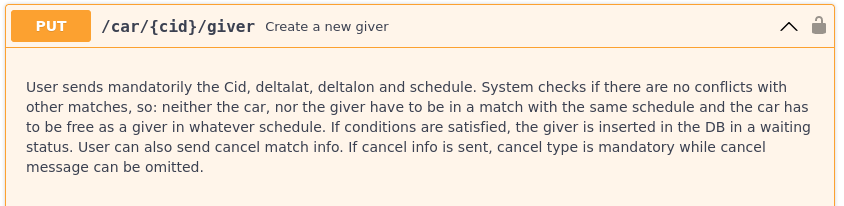
\includegraphics[width=1.1\linewidth]       {img/simulazione/giverbot/giver-request.png}
        \caption{Richiesta API per segnalarsi giver}
        \label{fig:giver request}
    \end{figure}
    \lstinputlisting[language=go]{Code/Simulazione/GiverBot/giver-request.go}


    \item \textbf{S1}: in questo secondo stato, il giver attende che il server stabilisca un match tra di lui ed un taker facendo polling all'API di match, la quale restituirà informazioni riguardanti il taker che memorizzeremo per utilizzarle nell'ultima fase. Inoltre, viene anche creato un secondo canale per catturare i segnali SIGKILL e SIGINTERRUPT cosicché la simulazione di questo bot sia interrompibile se non dovesse riuscire a trovare un match;

     \lstinputlisting[language=go]{Code/Simulazione/GiverBot/giver-wait-match.go}
    
    \item \textbf{S2}: ora che un match tra questo bot ed un altro è iniziato, il giver bot deve attendere il completamento del match da parte del taker. Il match terminerà quando il taker avrà raggiunto la posizione del giver, segnalandolo al server. Per verificare se il match è stato concluso viene fatto il polling della stessa chiamata API usata per attendere l'avvio del match;

    \lstinputlisting[language=go]{Code/Simulazione/GiverBot/giver-wait-end.go}
    
    \item \textbf{S3}: ora che il match è stato completato il giver deve lasciare il posto in cui ha parcheggiato al taker, il quale lo occuperà subito dopo;
    \lstinputlisting[language=go]{Code/Simulazione/GiverBot/giver-unpark.go}
    
    \item \textbf{S4}: in quest'ultimo stato i due bot che hanno appena concluso il match, hanno terminato il loro lavoro e sono quindi pronti a scambiarsi. Per fare questo scambio il giver salverà nel suo file CSV l'id del taker e della sua macchina memorizzati alla fine dello stato S1, al posto del suo record. In questo modo il giver non sarà più un giver mentre il taker lo sarà diventato. Allo stesso modo, il taker farà lo stesso scambio nel suo file CSV.

    \lstinputlisting[language=go]{Code/Simulazione/GiverBot/giver-trade.go}
    
\end{itemize}
Terminate tutte le 5 fasi ed effettuato lo scambio tra i due bot, il giver bot che ha appena concluso segnala di aver finito con il metodo \textbf{wg.Done}. Il programma attende quindi che tutti i bot terminino la loro esecuzione con \textbf{wg.Wait} \ref{fig:giver start}, controlla eventuali segnali SIGKILL e SIGINTERRUPT e ricomincia il caricamento di una nuova serie di giver bot \ref{fig:giver load}. 


\subsection{Taker Bot}\label{sec:taker-bot}
Come per il giver bot, il taker bot è il bot che simula il comportamento di un taker. Anche i taker utilizzano una struttura simile ai giver per rappresentare un singolo bot. Tra le informazioni memorizzate in questa struttura troviamo il suo nome, il suo id, l’id della sua macchina, lo schedule con il quale ha cercato un match, il timeslot in cui ha trovato un
match, le coordinate del giver con cui ha iniziato un match, le sue coordinate di partenza, l'id del trip che rappresenta il match e l'id della simulazione.

\lstinputlisting[language=go]{Code/Simulazione/TakerBot/taker-struct.go}

\subsubsection{Creazione e Inizio Simulazione}
La creazione dei bot necessari è identica a quella del giver bot \ref{fig:giver create}. \newline
Una volta che siamo sicuri dell'esistenza di almeno un bot, se ne è appena stato creato uno o era già presente nel file CSV, possiamo considerata iniziata una simulazione, salvandola quindi nel database.
\lstinputlisting[language=go]{Code/Simulazione/TakerBot/simulation-start.go}
\begin{figure}[H]
    \centering
    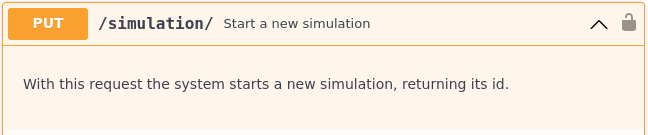
\includegraphics[width=1\linewidth]{img/simulazione/takerbot/simulazione-start-api.png}
    \caption{API per iniziare la simulazione}
    \label{fig:simulazione start api}
\end{figure}
Con abbastanza bot nel file CSV e la simulazione ufficialmente iniziata possiamo iniziare, come per il giver bot, un ciclo infinito per permettere un'esecuzione continua della simulazione fino all'interruzione da parte dell'utente. 

\subsubsection{Caricamento}\label{takerload}
Il caricamento dei bot necessari dal file CSV è simile a quello del giver bot con l'eccezione che questa volta verranno memorizzate, per ogni bot, anche l'id della simulazione ottenuto quando la simulazione è iniziata, e le coordinate di partenza del bot, le quali erano state salvate nel file CSV quando erano un giver oppure nel processo di creazione che, in questo caso, saranno delle coordinate di default inserite nel file di configurazione. Inoltre, al contrario dei giver bot, i taker non verranno parcheggiati una volta caricati.

\subsubsection{Ricerca Giver}
A questo punto abbiamo caricato tutti i bot necessari in una lista. Dobbiamo quindi cercare dei giver con cui effettuare dei match ed assegnare ad ogni giver trovato, uno dei taker appena caricati. \newline
Con la richiesta \textbf{requests.GetGiverList()}, ci verrà restituita una lista di giver bot disponibili per fare un match ed il loro schedule. Filtriamo ora tutti i giver trovati per cercare quelli compatibili con i nostri taker bot. Quelli compatibili per un match verranno salvati in una lista apposita ed assegnati, uno ad uno, ai taker bot necessari per soddisfarli tutti. Se dovessero essere presenti più taker bot che giver bot, quelli in eccesso verranno utilizzati in un prossimo ciclo della simulazione.

\lstinputlisting[language=go]{Code/Simulazione/TakerBot/find-giver.go}

Ora che ogni taker ha il suo giver con cui poter effettuare un match è finalmente possibile iniziare la simulazione nella quale ogni bot agirà indipendentemente dagli altri.\newline
A differenza dei giver bot, i taker bot faranno in seguito utilizzo di un' API esterna la quale ha un limite di due richieste contemporaneamente. Per questo motivo viene creato un semaforo condiviso tra tutti i bot in modo tale che soltanto due bot alla volta potranno fare quella richiesta.\label{takerstart}

\lstinputlisting[language=go]{Code/Simulazione/TakerBot/taker-start.go}

Similmente al giver bot, anche il taker controllera a questo punto se sono state intercettati segnali SIGKILL o SIGINTERRUPT ma questa volta, quando il segnale sarà intercettato, la simulazione verrà interrotta inserendo nella tupla del database una data di fine simulazione.
\begin{figure}[H]
    \centering
    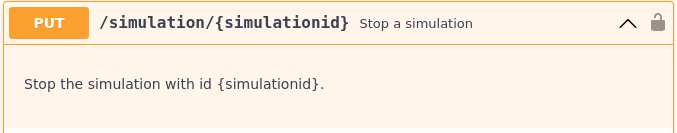
\includegraphics[width=1\linewidth]{img/simulazione/takerbot/simulazione-stop-api.png}
    \caption{API per interrompere la simulazione}
    \label{fig:simulazione stop api}
\end{figure}

\begin{figure}[H]
    \centering
    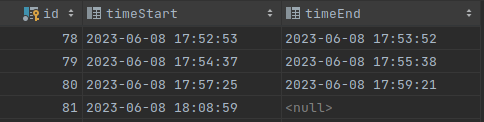
\includegraphics[width=0.8\linewidth]{img/simulazione/takerbot/simulazione-db.png}
    \caption{Simulazioni salvate nel database}
    \label{fig:simulazione db}
\end{figure}

\subsubsection{Simulazione del taker}

\begin{figure}[H]
    \centering
    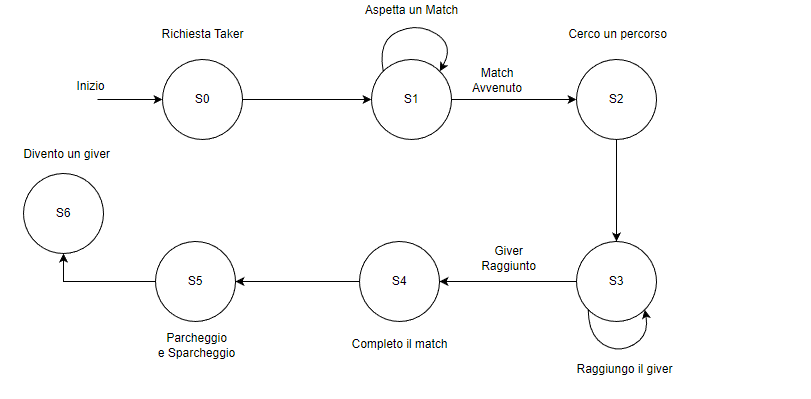
\includegraphics[width=1.2\linewidth]{img/simulazione/takerbot/taker-simulazione.png}
    \caption{Automa della simulazione di un taker bot}
    \label{fig:takerbot automa}
\end{figure}

Come possiamo vedere nella figura \ref{fig:takerbot automa}, la simulazione di un taker è composta da 7 stati diversi:
\begin{itemize}
    \item \textbf{S0}: in questo primo stato, il bot invia al server una richiesta per segnalarsi come taker. Con questa richiesta, il bot invia anche le sue coordinate, il suo range di ricerca e l'orario; 
    \begin{figure}[H]
        \centering
        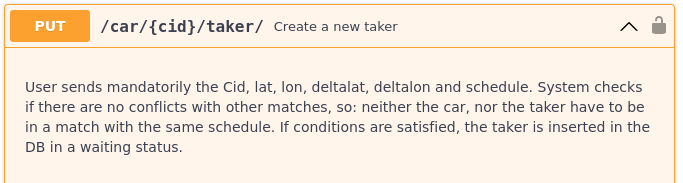
\includegraphics[width=1.1\linewidth]       {img/simulazione/takerbot/taker-request.png}
        \caption{Richiesta API per segnalarsi taker}
        \label{fig:taker request}
    \end{figure}
    \lstinputlisting[language=go]{Code/Simulazione/TakerBot/taker-request.go}


    \item \textbf{S1}: nel secondo stato, il taker attende che il server stabilisca un match tra di lui ed un giver facendo polling all'API di match, la quale restituirà informazioni riguardanti il giver che memorizzeremo per utilizzarle nell'ultima fase se c'è stato un match;

     \lstinputlisting[language=go]{Code/Simulazione/TakerBot/taker-wait-match.go}
    
    \item \textbf{S2}: ora che il match è iniziato, il taker deve trovare una strada da percorrere per raggiungere il giver. Viene quindi usata la funzione \textbf{requets.FindPath()}, la quale effettua delle richieste API a Project OSMR \cite{osmr} che restituirà un grande set di coordinate divise in segmenti, rappresentanti la strada più veloce che collega il taker con il giver. \newline
    Come accennato in precedenza, Project OSMR permette solo due richieste alla volta. Sfruttiamo quindi il semaforo creato per dare il lock alla funzione a solamente due bot per volta. \newline
    Per approfondire questa funzione vedasi la sezione \ref{FindPath};

    \lstinputlisting[language=go]{Code/Simulazione/TakerBot/taker-find-path.go}
    
    \item \textbf{S3} \label{follow-path}: in questo stato, il taker ha ottenuto un percorso valido per raggiungere il giver e non gli resta che seguirlo. Per dare un senso di realtà, il taker percorre ogni segmento dell'intero percorso in un tempo casuale, scelto tra il tempo massimo e minimo inseriti nel file di configurazione, moltiplicato per la lunghezza del segmento che si sta percorrendo. Questo implica che il taker impiegherà più tempo a percorrere un pezzo di strada lungo rispetto ad uno più corto.\newline
    Inoltre, salviamo nel database ogni set di coordinate raggiunte dal taker. Salvare queste coordinate sarà necessario per visualizzare il percorso di ogni match \ref{visualizzazioneWeb};
    
    \lstinputlisting[language=go]{Code/Simulazione/TakerBot/taker-follow-path.go}


    \item \textbf{S4}: una volta terminato il percorso da percorrere, il taker avrà raggiunto la posizione del giver e quindi il parcheggio che deve occupare. Deve quindi segnalare al server la sua intenzione di completare il match che a sua volta informerà anche il giver di poter lasciare il parcheggio;

    \lstinputlisting[language=go]{Code/Simulazione/TakerBot/taker-complete-match.go}

    \item \textbf{S5}: ora che il match è stato segnato come completato il giver starà lasciando il parcheggio. Il taker deve quindi occupare il parcheggio appena lasciato per poi lasciarlo subito dopo in modo tale da essere pronto per la sua prossima simulazione;

    \lstinputlisting[language=go]{Code/Simulazione/TakerBot/taker-park-unpark.go}
    
    \item \textbf{S6}: in quest'ultimo stato i due bot che hanno appena concluso il match sono pronti a scambiarsi. Per fare questo scambio il taker salverà nel suo file CSV l'id, l'id della macchina e la posizione del giver, al posto del suo record. In questo modo il taker non sarà più un taker mentre il giver lo sarà diventato. Allo stesso modo, il giver farà lo stesso scambio nel suo file CSV.

    \lstinputlisting[language=go]{Code/Simulazione/TakerBot/taker-trade.go}
    
\end{itemize}

Terminate tutte le 7 fasi ed effettuato lo scambio tra i due bot, il bot che ha appena concluso segnala di aver finito con il metodo \textbf{wg.Done}. Il programma attende quindi che tutti i bot terminino la loro esecuzione con \textbf{wg.Wait} \ref{takerstart}, controlla eventuali segnali SIGKILL e SIGINTERRUPT e ricomincia il caricamento di una nuova serie di taker bot \ref{takerload}. 


\subsubsection{Funzione Find Path}\label{FindPath}
In questa sezione vorrei approfondire la funzione FindPath.

\begin{lstlisting}[language=go]

func FindPath(giverLat,giverLon,takerLat,takerLon float64)(geo.PointSet,[]int,error){}

\end{lstlisting}
Come spiegato prima, questa funzione esegue delle richieste API a Project OSMR \cite{osmr} per ottenere un percorso da seguire in macchina che possa condurre il taker fino al giver. \newline
Per semplificare potremmo dividere la funzione in due parti:

\begin{itemize}
    \item \textbf{La richiesta}
    \item \textbf{Analisi del risultato}
\end{itemize}

Nella prima parte viene eseguita la richiesta ad OSMR sfruttando il client offerto dal pacchetto \textbf{github.com/gojuno/go.osrm} \cite{gojuno}.

\lstinputlisting[language=go]{Code/Simulazione/TakerBot/find-path-request.go}

Nella seconda parte analizziamo invece la risposta ricevuta dalla precedente chiamata.

\lstinputlisting[language=go]{Code/Simulazione/TakerBot/find-path-analysis.go}
Questa chiamata API ci restituisce un enorme quantità di coordinate, abbastanza da rappresentare alla perfezione ogni piccolo segmento di strada dell'intero percorso. Nella nostra simulazione non abbiamo però bisogno di rappresentare alla perfezione l'intero percorso considerando che il taker notifica la sua posizione ad ogni cambio di strada e che memorizzando nel database ogni set di coordinate raggiunte dal taker rischieremmo di avere un numero enorme di tuple per ogni match. Prendiamo quindi solamente la prima coordinata di ogni strada che compone il percorso in modo tale da avere una rappresentazione realistica del percorso, senza però occupare troppo spazio nel database. Memorizziamo inoltre la lunghezza (numero di coordinate) di ogni strada del percorso per usarla in seguito, limitandola però a 15 per non avere attese troppo lunghe. \newline
La funzione restituisce quindi il percorso che il taker dovrà seguire e la lunghezza di ogni segmento che lo compone in due array.


\subsection{Modifiche database}
Per poter memorizzare le simulazioni e distinguere i trip fatti da un bot da quelli fatti da un utente normale è risultato necessario fare delle modifiche al database.\newline
Per gestire al meglio le simulazioni, ho quindi aggiunto al database due nuove tabelle ed apportato modifiche ad alcune già esistenti.\newline
Ho innanzitutto aggiunto la nuova tabella \textbf{simulations}, la quale rappresenta tutte le simulazioni. In questa tabella possiamo capire se una simulazione è terminata oppure è in corso lasciando l'attributo \textbf{timeEnd} \say{null}. Inoltre, per indicare che un trip appartiene ad una simulazione, ho anche aggiunto l'attributo di chiave esterna \textbf{simulationId} nella tabella \textbf{trips}. \newline
Oltre le simulazioni, era anche necessario memorizzare tutte le coordinate di ogni trip fatto da un bot. Per questo motivo ho creato la tabella \textbf{simulated\_trip\_points} la quale contiene appunto tutte le coordinate legate ad un trip.


    \begin{figure}[H]
        \centering
        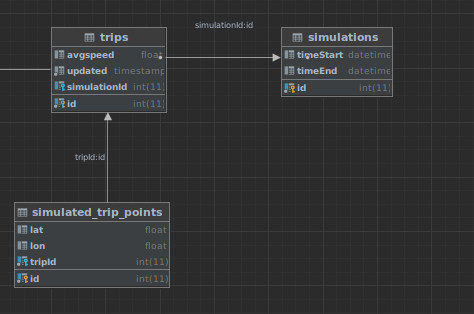
\includegraphics[width=1\linewidth]       {img/simulazione/db.png}
        \caption{Diagramma delle tabelle inerenti alle simulazione}
        \label{fig:db}
    \end{figure}

\subsection{Logger}
Nella simulazione viene fatto uso di un logger, il quale registra ogni azione commessa dai due programmi. Tramite l'uso del logger è possibile analizzare l'intera simulazione, mostrandoci ogni errore che può capitare durante l'esecuzione. 

    \begin{figure}[H]
        \centering
        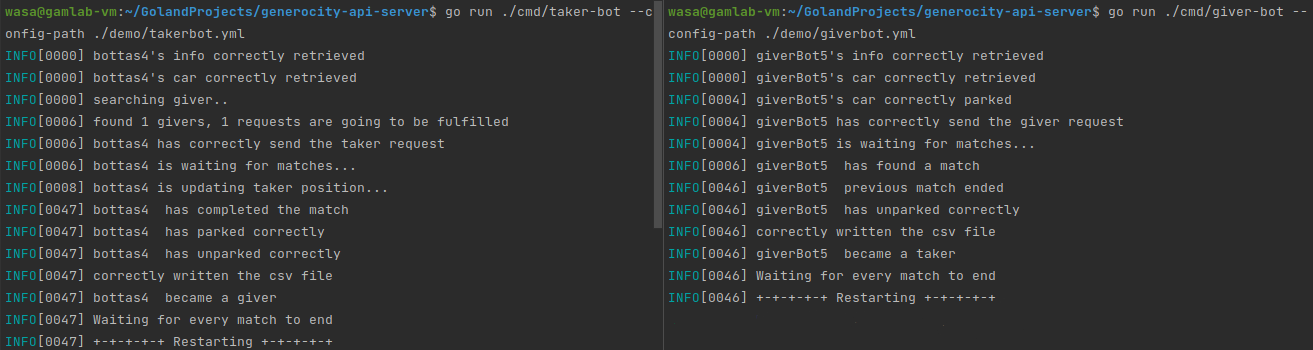
\includegraphics[width=1\linewidth]       {img/simulazione/logs.png}
        \caption{Log ottenuti durante una simulazione tra due bot}
        \label{fig:log}
    \end{figure}

\section{Visualizzazione Web}\label{visualizzazioneWeb}
Avendo una simulazione funzionante che salva anche tutte le informazioni necessarie per ricostruirla in seguito, è rimasto solo di visualizzarla su una mappa durante l'esecuzione. Per fare ciò ho realizzato una semplice pagina web in HTML che comunica con il programma tramite delle API appositamente realizzate. \newline

    \begin{figure}[H]
        \centering
        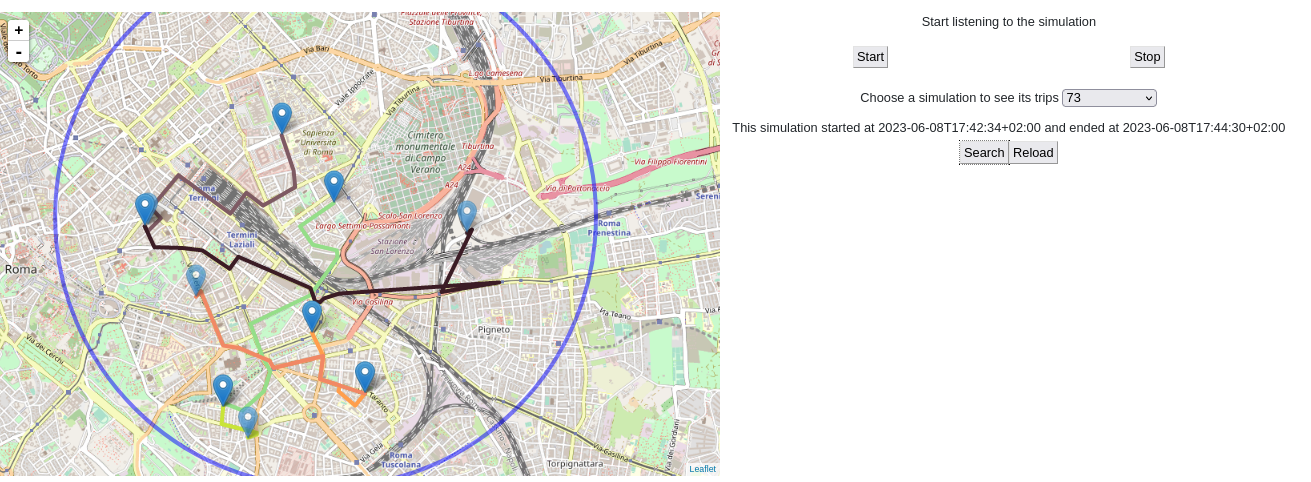
\includegraphics[width=1\linewidth]       {img/simulazione/web/oldSim.png}
        \caption{Visualizzazione web di una simulazione}
        \label{fig:oldSim}
    \end{figure}

Questa pagina sfrutta la mappa offerta dalla libreria JavaScript open-source Leaflet \cite{leafletjs}. Grazie a questa libreria è possibile mostrare una mappa con markers per indicare la posizione di tutti i bot ed il percorso che hanno seguito.

\subsubsection{Simulazione in tempo reale}
Una volta premuto il pulsante \say{Start}, la pagina inizia a fare richieste API al server ogni due secondi per ottenere le informazioni della simulazione in corso (se presente).

\begin{figure}[H]
    \centering
    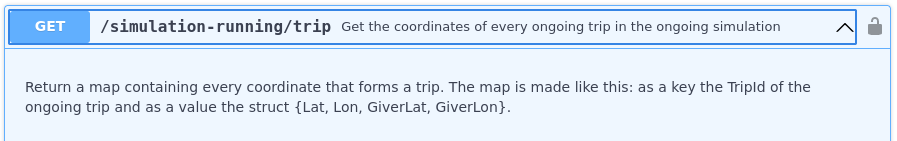
\includegraphics[width=1\linewidth]     {img/simulazione/web/runningGet.png}
    \caption{API per ottenere la simulazione in corso}
     \label{fig:runningGet}
\end{figure}

Se ci dovessero essere simulazioni in corso, l'API restituirà un JSON contenente tutti i trip in corso. Ogni elemento nel JSON sarà una coppia formata dall'id del trip ed un array di oggetti \textbf{MapPoints}. Questo array rappresenta tutte le coordinate di un trip salvate nel database dal taker mentre stava percorrendo la strada per raggiungere il giver (memorizzate in \ref{follow-path}). Insieme alle coordinate attuali, vengono passate anche le coordinate del giver da raggiungere così da poterlo mostrare sulla mappa.

\lstinputlisting[language=go]{Code/Simulazione/Web/MapPoints.go}

\begin{figure}[H]
    \centering
    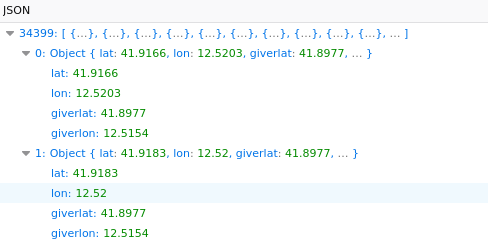
\includegraphics[width=1\linewidth]     {img/simulazione/web/response.png}
    \caption{Esempio di risposta}
     \label{fig:runningResponse}
\end{figure}

Una volta ricevuta una risposta, tutti i trip in corso vengono visualizzati sulla mappa ed aggiornati ogni due secondi finché non verrà premuto il pulsante \say{Stop}.\newline
Possiamo distinguere tre tipi di marker:

\begin{itemize}
    \item \textbf{Partenza Taker} : il marker più scuro;
    \item \textbf{Posizione Taker} : il marker semitrasparente;
    \item \textbf{Posizione Giver} : il marker leggermente più chiaro di quello del taker.
\end{itemize}


\begin{figure}[H]
    \centering
    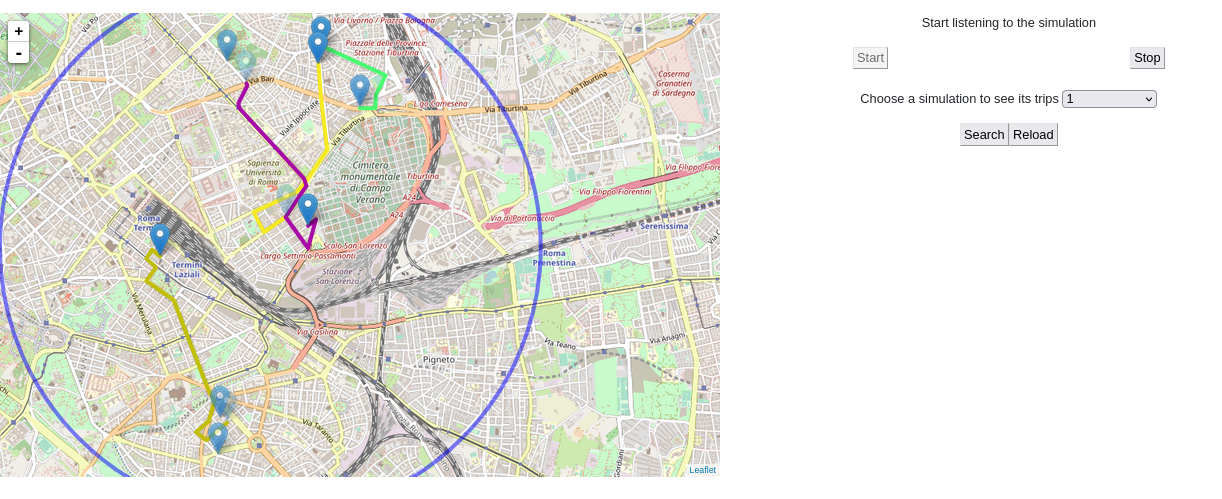
\includegraphics[width=1\linewidth]     {img/simulazione/web/runningTrip.png}
    \caption{Simulazione in corso}
     \label{fig:runningTrip}
\end{figure}

\subsubsection{Vecchie simulazioni}
Tramite questa pagina è anche possibile visualizzare simulazioni ormai terminate. \newline
Appena la pagina viene caricata, viene fatta una richiesta API al server per ottenere l'id e la data di tutte le simulazioni già terminate. Questo elenco appena ottenuto viene inserito nel menù a tendina, il quale permetterà all'utente di selezionare una qualsiasi simulazione, mostrando anche la data in cui è stata svolta. 

\begin{figure}[H]
    \centering
    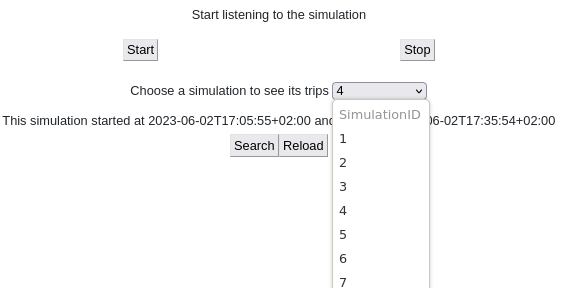
\includegraphics[width=1\linewidth]     {img/simulazione/web/simulationSelect.png}
    \caption{Menù a tendina}
     \label{fig:simulationSelect}
\end{figure}

Una volta scelta una simulazione, basterà premere il pulsante \say{Search} per visualizzare tutti i trips svolti durante quella simulazione. \ref{fig:oldSim}



\end{document}